\documentclass[11pt]{article}
\usepackage[margin=0.9in]{geometry}
\usepackage[T1]{fontenc}
\usepackage{newtxtext,newtxmath}
\usepackage{microtype,graphicx,booktabs,tabularx,longtable,array,enumitem}
\usepackage{amsmath,mathtools}
\usepackage[font=small,labelfont=bf]{caption}
\usepackage[section]{placeins}
\usepackage{xcolor,xurl,hyperref,fancyhdr}
\definecolor{navy}{HTML}{245B85}
\hypersetup{colorlinks=true,linkcolor=navy,citecolor=navy,urlcolor=navy,pdftitle={LLM Inference Serving: Foundations, Systems, and the Case for ATFM},pdfauthor={ATFM project}}
\setlength{\headheight}{14pt}
\pagestyle{fancy}\fancyhf{}\fancyhead[L]{\small LLM inference serving}\fancyhead[R]{\small Technical background}\fancyfoot[C]{\thepage}
\renewcommand{\topfraction}{0.9}
\renewcommand{\textfraction}{0.08}
\renewcommand{\floatpagefraction}{0.65}
\setlength{\parskip}{4pt}\setlength{\parindent}{1em}
\setlist{itemsep=3pt,topsep=5pt}
\newcommand{\E}{\mathbb{E}}
\newcommand{\Prb}{\mathbb{P}}
\newcommand{\ind}{\mathbf{1}}
\newcommand{\fig}[4]{\begin{figure}[htbp]\centering\includegraphics[width=#2\linewidth]{figures/#1.pdf}\caption{#3}\label{fig:#4}\end{figure}}
\newcommand{\takeaway}[1]{\begin{quote}\textbf{Practical consequence.} #1\end{quote}}
\begin{document}
\begin{titlepage}
\vspace*{1.0cm}
{\color{navy}\large ATFM TECHNICAL BACKGROUND\par}
\vspace{0.7cm}
{\Huge\bfseries LLM Inference Serving\par}
\vspace{0.4cm}
{\LARGE Foundations, systems, and the case for anticipatory control\par}
\vspace{0.9cm}
{\large KV caches, vLLM, LMCache, distributed serving, and agent workloads\par}
\vspace{1cm}
\textbf{Research cutoff: 28 September 2026}\par
Repository baseline: \texttt{900d63b}, following the verified core refactor.\par
\vspace{0.7cm}
\begin{abstract}
An LLM service converts a stream of variable-length, stateful computations into
latency-constrained responses. Efficient matrix multiplication is necessary, but
so are memory allocation, batching, cache reuse, data movement, routing, and
admission control. Agent workloads add a further complication: a session can
stop generating tokens while a tool runs, yet return with a large reusable
context. The best immediate request decision need not be the best session or
fleet decision.

This paper develops the serving stack from first principles, derives the main
memory, compute, bandwidth, and queueing relationships, and maps major research
and open-source systems onto the problems they solve. It covers paged attention,
continuous batching, prefix reuse, cache tiers, prefill/decode disaggregation,
parallelism, compression, and program-aware scheduling. It then defines ATFM's
potential contribution precisely: using observations available before an agent's
next request to estimate future demand and inform bounded control actions.
Existing systems already address substantial parts of this problem. The paper
therefore gives both the case for ATFM and conditions under which it adds no
value, with a comparison and evaluation plan that can falsify the hypothesis.
All numerical illustrations are derived examples unless explicitly identified as
repository measurements. No new GPU serving benchmark is claimed.
\end{abstract}
\vfill
\noindent\small Primary-source survey and engineering synthesis. Living documentation
was inspected at the cutoff date; deployment APIs must be pinned and tested.
\end{titlepage}
\tableofcontents
\clearpage
\section{The problem the serving stack actually solves}
\label{sec:orientation}
A model checkpoint describes a computation. A serving system must decide when,
where, and with what retained state to perform that computation for many users
at once. Two prompts of the same length can have very different service costs:
one may reuse a cached prefix on an idle GPU; another may need a full prefill,
a remote transfer, or admission behind a long queue. A fleet with fast kernels
can still deliver poor latency if it repeatedly recomputes old contexts or
routes requests to an overloaded cache-rich worker.

An agent makes the problem more temporal. A coding agent may generate a command,
wait for a test suite, append its output, and ask the model again. During the
wait, the GPU sees no active decode for that session. Nevertheless, retaining
some state may save work when the tool finishes. Retaining everything can also
prevent other sessions from making progress. The decision requires the cost of
keeping state, the cost of losing it, and the likely time until reuse.

\subsection{A map of responsibilities}
Figure~\ref{fig:stack} distinguishes six layers. The application determines
semantics and dependencies. A gateway enforces request limits and routes work.
An inference engine schedules token computation and manages active state.
Kernels implement tensor operations. A cache service extends where reusable
state can live. A tool runtime executes non-LLM work. A single product can span
several layers; the boundaries describe responsibilities, not mandatory processes.

\fig{stack}{0.82}{A conceptual serving stack. Arrows denote request or data exchange,
not a mandated implementation. ATFM primarily concerns the information and policy
between applications and serving; it does not replace GPU kernels.}{stack}

\begin{table}[htbp]\centering\small
\caption{Questions that belong to different layers.}
\begin{tabularx}{\linewidth}{@{}lXX@{}}\toprule
Layer & Main question & Typical cost of a wrong decision\\\midrule
Kernel & How do these tensors execute efficiently? & Extra device IO or compute\\
Engine & Which token work fits this iteration? & Stalls, preemption, wasted capacity\\
Cache & Which reusable state should exist where? & Recompute, transfer, occupied memory\\
Router & Which worker should receive this request? & Queueing or lost locality\\
Admission & Should this work enter now? & Overload or unnecessary delay\\
Agent control & What is likely to arrive after a tool? & Missed preparation or wasted reservation\\\bottomrule
\end{tabularx}\end{table}

\subsection{How to read this paper}
Readers new to serving should start with the equations and worked memory example
in Section~\ref{sec:fundamentals}, then the engine and cache sections. Readers
already operating vLLM can focus on cache movement, agent scheduling, and the
ATFM assessment. The appendix provides notation, terminology, a diagnosis guide,
and a reading sequence. Equations are models with stated assumptions, not
universal performance predictors.

The survey is broad but deliberately bounded. It emphasizes autoregressive
transformer inference, open serving infrastructure, and systems relevant to
agent traffic. Training, model-quality leaderboards, mobile inference, and every
proprietary platform are outside scope. ``State of the art'' means the relevant
research frontier and actively documented mechanisms, not one universally
fastest system. Published comparisons differ in hardware, model, workload,
cache warmness, implementation generation, and latency constraints. Their
headline speedups cannot be put in one league table.

\subsection{Three kinds of evidence}
\textbf{Established mechanism} means a cited paper or implementation documents
how a technique works. \textbf{Analytical illustration} means a derivation or a
synthetic example in this paper, with explicit numbers and assumptions.
\textbf{ATFM evidence} means a result recorded in this repository. A source's
reported benchmark is evidence for that source's configuration, not an ATFM
result. Recent preprints are marked as such; living documentation has an access
date. We use primary papers and project documentation, and avoid reproducing
vendor peak-throughput rankings.

The central hypothesis is intentionally narrower than ``agents need better
serving'': conditional information about a paused session can improve a future
resource decision enough to pay for obtaining and acting on that information.
A forecast with lower statistical error is not sufficient. The decision must
change, complete before it matters, and improve a user-relevant outcome.

\section{From attention to compute, memory, and latency}
\label{sec:fundamentals}
\subsection{What is stored in a KV cache?}
For a single attention head, let a token's representation be projected into a
query $q$, key $k$, and value $v$. Given a prefix of length $T$, causal attention
for its newest token has the form
\begin{equation}
 o_T=\operatorname{softmax}\!\left(\frac{q_T K_{1:T}^{\mathsf T}}{\sqrt{d_h}}\right)V_{1:T}.
 \label{eq:attention}
\end{equation}
The keys determine how strongly earlier positions are attended to; values
provide the content combined by those weights. This is the standard
scaled-dot-product attention construction~\cite{transformer}. The cache stores
previously computed keys and values at the required layers. It is neither the
model's learned weights nor a cache of finished textual answers.

For a causal model with an unchanged prefix, earlier hidden states do not depend
on future tokens. Their keys and values therefore need not be recomputed when
one token is appended. The new query must still attend to the appropriate old
state. Caching removes repeated prefix construction; it does not make reading
or attending over the prefix free. Queries normally need not be retained for
future autoregressive steps.

A cache entry has a computational identity. Matching text alone is insufficient
if model weights, adapters, tokenization, positional treatment, or multimodal
inputs differ. Reusing state under the wrong identity can silently change the
answer. Likewise, the KV for a passage following one prefix generally differs
from its KV following a different prefix. Exact prefix reuse and arbitrary
passage reuse are distinct mechanisms.

\subsection{Prefill and decode are different workloads}
During \emph{prefill}, the model processes known prompt tokens. Many token
projections and feed-forward operations can execute together as matrix-matrix
operations. During ordinary \emph{decode}, the next token is unknown until the
previous step completes. Each active sequence contributes roughly one new token
to an iteration, although speculative methods alter this unit of work.

Let $L$ be layers, $T$ prompt tokens, $d$ hidden width, and $H_qd_h=d$ for an
ordinary attention configuration. Ignoring architecture-dependent constants,
a dense model's prefill work has the form
\begin{equation}
 F_{\mathrm{prefill}}=\Theta(LTd^2)+\Theta(LT^2d).
 \label{eq:prefill}
\end{equation}
The first term collects projections and feed-forward computation, assuming its
intermediate width scales with $d$; the second is dense attention. A cached
single-token decode step at context length $t$ has work
\begin{equation}
 F_{\mathrm{step}}=\Theta(Ld^2)+\Theta(Ltd).
\end{equation}
For $U$ new output tokens after a $T$-token prompt, the attention contribution
sums as
\begin{equation}
 \sum_{u=0}^{U-1}\Theta(L(T+u)d)
 =\Theta\!\left(Ld\left(UT+\frac{U(U-1)}{2}\right)\right).
 \label{eq:decode}
\end{equation}
These expressions explain why a single cached decode step is linear in context
length while a long generation still accumulates a quadratic output-length
term. A deliberately naive implementation that reruns full dense attention over
the entire growing prefix at every step can accumulate cubic work in final
sequence length. That is not how a normal cached inference engine should run.
They are arithmetic counts, not wall-clock predictions: batching, memory
traffic, collective communication, and kernel utilization matter.

FlashAttention tiles exact attention to reduce traffic to high-bandwidth memory
and avoid materializing the full attention matrix there. It does not turn dense
attention into a linear-arithmetic algorithm~\cite{flash}. FlashAttention-3
uses hardware-oriented overlap and low-precision techniques~\cite{flash3}.
FlashInfer focuses on flexible, efficient inference kernels across cache
layouts and dynamic serving patterns~\cite{flashinfer}. These optimizations are
complementary to scheduling: a better admission policy cannot recover all the
performance lost by an unsuitable attention backend.

\subsection{The cache-size equation}
For a uniform full-attention model, an unsharded sequence's KV payload is
\begin{equation}
 M_{\mathrm{KV}}(T)=2LH_{kv}d_hbT,
 \qquad m_{\mathrm{token}}=2LH_{kv}d_hb,
 \label{eq:kvbytes}
\end{equation}
where $H_{kv}$ is the number of key/value heads, $b$ bytes per stored scalar,
and the leading two counts keys and values. This excludes allocator metadata,
quantization scales, temporary buffers, and replication. With $B$ independent
sequences of lengths $T_i$, payload is $m_{\mathrm{token}}\sum_iT_i$ before
sharing or architectural exceptions.

Multi-head attention (MHA) uses separate KV heads for query heads. Multi-query
attention (MQA) shares one KV head across queries~\cite{mqa}. Grouped-query
attention (GQA) sits between them, with several query heads sharing a KV
head~\cite{gqa}. Reducing $H_{kv}$ changes model architecture and its stored
representation; it is not merely a runtime eviction policy.

\paragraph{Worked example.}
Take an illustrative $L=32$, $H_{kv}=8$, $d_h=128$, and $b=2$. Then
\begin{align}
 m_{\mathrm{token}}&=2\cdot32\cdot8\cdot128\cdot2
 =131{,}072\ \mathrm{bytes}=128\ \mathrm{KiB},\\
 M_{\mathrm{KV}}(8192)&=1\ \mathrm{GiB}.
\end{align}
Sixty-four independent 8192-token contexts consume 64 GiB of payload before
weights and other allocations. A hypothetical 80 GiB device with 20 GiB of
weights and 8 GiB reserved for runtime overhead leaves 52 GiB, so only 52 such
contexts fit under this simplified arithmetic. This is a memory upper bound,
not a recommended concurrency or measured GPU capacity. Decode throughput and
latency may impose a lower limit.

\fig{kv-growth}{0.91}{Derived KV payload for an illustrative uniform model.
Changing the number of KV heads changes the slope; paging changes allocation
waste rather than the payload slope. No hardware was benchmarked.}{kvgrowth}

\subsection{Where the simple formula stops applying}
Multi-head latent attention, introduced in DeepSeek-V2, stores a compressed latent
representation rather than the ordinary full per-head KV tensors~\cite{mla}.
Its memory formula must include that representation and any positional state;
substituting an arbitrary small $H_{kv}$ into Equation~\ref{eq:kvbytes} is not a
general MLA estimator. Sliding-window layers retain a bounded attention window;
hybrid models may mix full attention, local attention, and recurrent state.
vLLM's hybrid cache manager explicitly handles different layer groups and their
cache-hit rules~\cite{hybrid}.

Tensor parallelism can shard cache heads, but heads or other state may be
replicated depending on the model and parallel degree. Pipeline parallelism
partitions layers. Context parallelism partitions sequence work/state and
introduces communication. Always distinguish total cluster bytes from bytes on
the busiest rank. Dividing a global KV estimate by GPU count is valid only if
the actual layout shards it evenly. A controller should consume measured
per-worker capacity and layout metadata rather than infer them from a model's
parameter count.

\subsection{The roofline view: what limits one iteration?}
A useful lower-bound model is
\begin{equation}
 t_{\mathrm{iter}}\gtrsim
 \max\left(\frac{F}{P_{\mathrm{eff}}},
           \frac{D_{\mathrm{HBM}}}{B_{\mathrm{HBM,eff}}},
           \frac{D_{\mathrm{link}}}{B_{\mathrm{link,eff}}}\right).
 \label{eq:roofline}
\end{equation}
$F$ is floating-point work; $D$ terms are transferred bytes; $P$ and $B$ are
achievable rates for this workload, not device marketing peaks. Real latency
also includes launches, synchronization, queueing, and portions that cannot
overlap. Adding all three ratios overestimates fully overlapped work; taking
only their maximum underestimates serial dependencies. The execution trace
determines which is appropriate.

Small-batch dense decode often pays heavily to read weights and KV for few new
tokens. Batching amortizes weight traffic across more tokens, but adds KV reads
and can increase per-iteration latency. Large prefill can exploit compute well,
yet long-context attention or distributed communication may become limiting.
``Prefill is compute-bound and decode is memory-bound'' is a useful first
hypothesis, not a property true for every shape, model, or device.

Arithmetic intensity is $I=F/D_{\mathrm{HBM}}$. In a simplified roofline,
achievable FLOPs/s is bounded by $\min(P_{\mathrm{eff}}, I B_{\mathrm{HBM,eff}})$.
Optimizing Python dispatch will have little effect while a long GPU kernel is
dominant and well fed. It can matter enormously when short iterations wait for
CPU scheduling or when a control service saturates a core. These are different
critical paths and require different measurements.

\subsection{Latency metrics and useful throughput}
Let $a_i$ be request arrival, $f_i$ first-token delivery, $z_i$ last-token
delivery, and $U_i$ the number of output tokens. Then
\begin{align}
 \mathrm{TTFT}_i &= f_i-a_i,\\
 \mathrm{TPOT}_i &= \frac{z_i-f_i}{U_i-1}\quad(U_i>1).
\end{align}
Individual inter-token latencies (ITLs) are adjacent delivery gaps. TPOT is an
average over those gaps and can hide a single long stall. TTFT includes queueing,
frontend work, cache retrieval, prefill, and delivery; it is not a direct prefill
kernel timer. Client-observed latency also includes transport and buffering.

For horizon $H$, define request goodput under a chosen joint SLO as
\begin{equation}
 G=\frac{1}{H}\sum_i\ind\{\mathrm{success}_i,
 \mathrm{TTFT}_i\le\tau_f,\ \mathrm{TPOT}_i\le\tau_o\}.
 \label{eq:goodput}
\end{equation}
Report the definition of success, errors, offered load, and rejected requests.
A system that rejects difficult work can appear to have excellent latency while
serving few users. Token throughput alone can favor longer outputs or a changed
workload mix. For agents, whole-job completion time and task success are needed
in addition to per-call metrics.

\section{Inside an inference engine}
\label{sec:engines}
\subsection{From static batches to iteration-level scheduling}
In a static batch, requests can remain tied together until the longest member
finishes. A request producing ten tokens then wastes potential participation
while another produces a thousand. Iteration-level scheduling chooses the active
set again between model iterations, allowing finished requests to leave and
new work to enter. Orca established this design for generative-model
serving~\cite{orca}. ``Continuous batching'' is the common operational term.

Consider three requests with output lengths 2, 5, and 3. In a deliberately
simplified model where a three-slot iteration has constant cost, a fixed batch
runs five iterations for ten useful token updates out of fifteen possible
slots. A dynamic scheduler can fill vacated slots with new requests. This
example demonstrates available scheduling opportunity, not a $15/10$ speedup:
real iteration time changes with batch composition, prompt work, and cache
length. The scheduler also needs free state capacity before admitting work.

The engine's queue is not interchangeable with the external gateway queue.
Once admitted, a request may consume KV blocks and compete for token budget.
Holding a request outside the engine avoids some of that pressure but adds
waiting before execution. A useful gateway admission policy must understand
what the engine can already do, otherwise it can reduce batching and leave the
GPU idle.

\subsection{PagedAttention and the vLLM memory model}
The foundational vLLM design maps a sequence's logical KV blocks to physical
blocks allocated as needed. Blocks do not have to be adjacent in GPU memory.
This reduces large reservations and external fragmentation, and permits shared
blocks with reference counting and copy-on-write behavior~\cite{paged}.
Paging does not compress the tensors in Equation~\ref{eq:kvbytes}.

For a block capacity of $p$ tokens, sequence $i$ with $T_i$ tokens requires
$\lceil T_i/p\rceil$ blocks. Its unused tail is
\begin{equation}
 w_i=p\left\lceil T_i/p\right\rceil-T_i,\qquad 0\le w_i<p.
\end{equation}
Ignoring shared blocks, tail waste is less than $Bp$ token slots for $B$
sequences. Larger blocks reduce some metadata and indexing overheads but
coarsen allocation and reuse; smaller blocks can reduce unused tails while
increasing management work. These are design tradeoffs, not a universal best
block size. The appropriate choice also depends on the attention backend and
model's supported layouts.

\fig{papers/vllm}{1.0}{vLLM's original block-table translation diagram:
logical token blocks map to noncontiguous physical KV blocks. Reproduced from
Kwon et al.~\cite{paged}, Figure 6, arXiv:2309.06180v1, CC BY 4.0;
scaled and format-converted only.}{paging}

vLLM's versioned prefix-cache design identifies full blocks using a chain of
hashes over prior-prefix identity, current tokens, and relevant extra identity
fields. A new request can reuse a matching prefix; reference counts and a free
block structure distinguish currently used from evictable blocks~\cite{prefix}.
A prefix can be logically cached yet be evicted when space is needed. An active
reference protects state required by a current computation; retaining a
finished session's state is a separate policy problem.

\paragraph{Walkthrough: two related prompts.}
Suppose prompts are ``system + repository + task A'' and ``system + repository +
task B''. If tokenization and all computational identity match through the
repository portion, those prefix blocks can be reused. If the first differing
token is inside a block, a block-level implementation's reuse boundary may be
before that token. Hash lookup is not a semantic similarity search. Changing a
system instruction near the front can invalidate later exact-prefix reuse even
when most natural-language content looks similar.

\subsection{vLLM V1: token budgets and host overhead}
The V1 guide describes a unified scheduler assigning token counts per request,
rather than entirely separate scheduling abstractions for prompt and output
phases. This supports composing chunked prefill, prefix caching, and speculative
work within a token-budget model~\cite{v1}. The abstraction matters because the
engine can control work more finely than a gateway that only counts requests.
An 80-token prompt and an 80,000-token prompt are not equal demand.

A conceptual budget is
\begin{equation}
 \sum_{i\in\mathcal A}n_i^{\mathrm{scheduled}}\le K,
 \qquad M_{\mathrm{active}}+M_{\mathrm{reserved}}\le M_{\mathrm{KV,budget}}.
\end{equation}
A token count is only a proxy for work: decode at long context has a different
cost from a short-context token, and full, local, and latent attention differ.
The hardware ultimately constrains time and memory, not abstract token units.

The host still tokenizes, validates requests, maintains scheduling metadata,
prepares tensors, and processes outputs. A model server can use Python at the
orchestration layer while kernels and collectives execute in compiled code.
The relevant question is whether Python lies on the measured critical path.
Moving every component to Rust does not change the amount of KV data read by a
GPU or transferred over a link. Removing repeated scans, redundant RPCs, or
avoidable serialization can matter before a language change does.

\subsection{Chunked prefill and interference}
A large prefill inserted among active decodes can delay their next tokens.
Chunking divides prompt work across iterations, placing a bound on how much
prefill competes with decode at once. Sarathi-Serve develops scheduling around
chunked prefills to manage this throughput/latency tension~\cite{sarathi}.

Let a chunk have $c$ tokens and estimated execution time $t_p(c,B,T)$ under the
current decode set. A conceptual ITL budget imposes
\begin{equation}
 t_d(B,T)+t_p(c,B,T)+t_{\mathrm{other}}\le\tau_{\mathrm{ITL}}.
\end{equation}
This additive approximation is conservative when work overlaps and optimistic
when it ignores interference. Smaller $c$ creates more scheduling boundaries
and may hurt compute efficiency. Larger $c$ can improve prompt throughput while
worsening decode tail gaps. Adaptive chunking requires measured response surfaces,
not simply choosing the smallest chunk.

\subsection{Other engine designs and why comparison matters}
\textbf{SGLang.} Its original work combines structured LLM-program execution
with RadixAttention, representing reusable prefixes in a radix-tree-oriented
cache~\cite{sglang}. This is an alternative organization of prefix reuse, not
an absence of memory constraints. Its current HiCache design extends reuse
beyond GPU memory; Section~\ref{sec:hierarchy} separates that layer from the
original engine mechanism.

\textbf{TensorRT-LLM.} The documented KV subsystem includes block pools, reuse,
secondary-memory offload, and prioritized eviction. Retention can attach
priorities to token ranges~\cite{trt}. Therefore a blanket statement that
``engines expose no retention controls'' is incorrect. ATFM must discover which
control is available in the deployed backend and compare against that engine's
best native retention policy.

\textbf{vAttention.} The memory-management paper with this name keeps the
virtual address layout contiguous while mapping physical GPU memory on demand
using CUDA virtual-memory APIs~\cite{vattention}. It addresses fragmentation
without requiring the same non-contiguous virtual layout as PagedAttention.
This paper is distinct from a later sparse-attention project with the same
name. The broader lesson is that block paging is one way to manage growing
state, not a mathematical prerequisite for efficient inference.

\subsection{Speculation, quantization, and parallel execution}
Speculative decoding generates candidate tokens with a cheaper draft process
and verifies them using the target model. With the appropriate acceptance and
correction algorithm it can preserve the target sampling distribution~\cite{spec}.
A simple throughput comparison is
\begin{equation}
 t_{\mathrm{effective\ token}}\approx
 \frac{t_{\mathrm{draft}}(k)+t_{\mathrm{verify}}(k)+t_{\mathrm{control}}}
      {\E[A(k)]},
\end{equation}
where $A(k)$ counts emitted tokens per round under the exact implementation,
including any additional verified token. Acceptance, draft overhead, available
batching, and memory use determine whether the method helps. A request-level
capacity estimator must not assume one target forward pass always equals one
emitted token.

Weight quantization reduces model storage/traffic; KV quantization reduces
sequence-state traffic. They alter different terms in the budget. KIVI studies
asymmetric low-bit quantization of keys and values~\cite{kivi}; low-bit cache
storage requires numerical-quality evaluation, scale metadata, and suitable
kernels. A factor-of-eight reduction in scalar bit width does not imply an
end-to-end factor-of-eight memory or latency reduction.

Parallelism redistributes work rather than removing it. Tensor parallelism
splits operations and adds collectives; pipeline parallelism splits layers and
can suffer bubbles; data parallelism creates independent model replicas and
needs routing; context parallelism spreads long sequence work; expert parallelism
routes mixture-of-experts tokens among expert shards. A fleet may combine them.
A cache-local routing decision that ignores collective topology can be worse
than a small cache miss on a better-connected worker group.

\takeaway{Before adding a higher-level controller, establish a tuned engine
baseline with continuous batching, appropriate kernels, realistic token budgets,
and the native cache/reuse features supported by the chosen model. ATFM should
be evaluated on top of that baseline, not credited for optimizations already
available in it.}

\section{Cache hierarchies, movement, and distributed serving}
\label{sec:hierarchy}
\subsection{A cache hit is a location-dependent event}
A prefix can be present on the destination GPU, retained in host memory, stored
on local SSD, or available at another machine. These cases all avoid some
recomputation but have different latency and resource costs. A remote hit may
be slower than local recomputation. A GPU hit may still wait behind another
request. A cache metadata hit is not proof that the tensors are ready for an
attention kernel.

For cache payload $M$, a useful restore model is
\begin{equation}
 t_{\mathrm{restore}}=t_{\mathrm{lookup}}+t_{\mathrm{queue}}+
 t_{\mathrm{setup}}+\frac{M}{B_{\mathrm{effective}}}+t_{\mathrm{layout}}+
 t_{\mathrm{sync}}.
 \label{eq:restore}
\end{equation}
The terms include object lookup, waiting for IO resources, transfer setup,
effective bandwidth, tensor layout conversion, and synchronization. Multiple
hops may overlap or serialize. Bottleneck link bandwidth is an optimistic
starting point, not necessarily the end-to-end rate. A distributed service must
also reserve destination capacity before advertising completed placement.

\fig{hierarchy}{0.86}{A conceptual KV hierarchy. Storage tiers hold reusable
state; the inference engine owns the state required for active attention.
Metadata/control paths are dashed. Product-specific tier names are not universal:
SGLang HiCache and LMCache use different L1/L2 terminology.}{hierarchy}

\paragraph{Restore versus recompute.}
A local decision compares completion costs, not merely existence:
\begin{equation}
 t_{\mathrm{restore}}+\Delta t_{\mathrm{interference}}
 < t_{\mathrm{recompute}}+\Delta t_{\mathrm{alternative\ queue}}.
 \label{eq:break-even}
\end{equation}
The extra terms matter when restores congest a link or recomputation occupies a
GPU that could serve other requests. For illustration, transferring 1 GiB at
25 GiB/s takes 40 ms before overhead; at 8 GiB/s it takes 125 ms. If fixed
overhead is 1 ms and recomputation costs 150 ms, both may help in isolation.
At 2 GiB, the slower path is already 251 ms. These rates and the recomputation
cost are assumptions, not device specifications or measurements.

\fig{transfer}{0.91}{Analytical restore-time curves from Equation~\ref{eq:restore}
with all terms except setup and transfer set to zero. The horizontal line is an
assumed recomputation cost. Queueing or layout conversion moves the crossover.}{transfer}

\subsection{LMCache: externalizing reusable inference state}
LMCache provides a cache layer that extracts, retains, retrieves, and exchanges
KV state around inference engines. Its technical report describes reuse across
requests and engines, prefill/decode transfers, batched movement, IO/compute
pipelining, and control APIs~\cite{lmcache}. It is not an LLM, tokenizer, or
replacement for the engine's attention scheduler. External cache capacity is
useful only if the correct state can be retrieved at a cost lower than the
alternative.

\begin{figure}[htbp]
\centering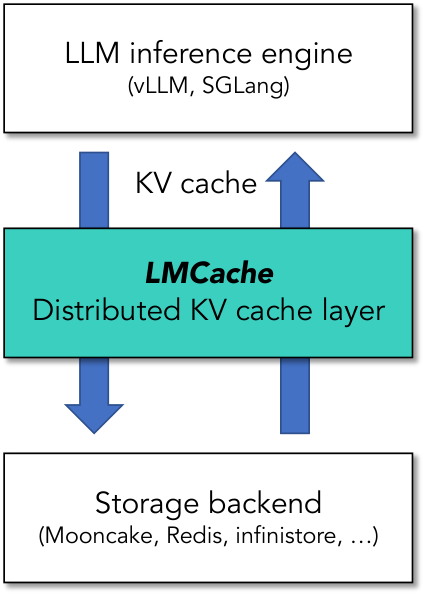
\includegraphics[width=0.52\linewidth]{figures/papers/lmcache.png}
\caption{LMCache's technical-report architecture connects inference engines to
storage and transport backends. Reproduced from Liu et al.~\cite{lmcache},
Figure 5, arXiv:2510.09665v2, CC BY 4.0; scaled only. This depicts the report's
architecture; the current multiprocess implementation is discussed below.}
\label{fig:lmcache-original}
\end{figure}

The current multiprocess architecture documentation places cache management in
a separate server. A storage manager composes local memory management, secondary
storage adapters, and asynchronous store, prefetch, and eviction controllers.
The documented local manager can be backed by CPU DRAM or a GPU-direct-storage
NVMe slab~\cite{lmp}. Therefore describing every LMCache deployment as ``a
Python dictionary of CPU tensors inside vLLM'' is both incomplete and stale.
A deployment must specify its mode, cache ownership, transport, storage backend,
and connector versions.

A conceptual read path is: identify a reusable prefix; discover available
objects; obtain valid access/retention while transferring them; populate the
engine's expected representation; wait for readiness at the required layer or
batch boundary; compute the unmatched suffix. A write path must decide when
and how much completed state to retain. These are generic correctness steps,
not a claim that a particular LMCache release exposes one API per step.

\paragraph{The integration contract that ATFM must verify.}
The legacy in-process controller page is now explicitly deprecated in favor of
multiprocess mode~\cite{llegacy}. Its pin API identifies tokens, an instance,
and a storage location, returning an operation event identifier; the documented
example pins a CPU backend~\cite{lpin}. That does not establish an engine-HBM
reservation, nor does an accepted asynchronous operation prove transfer
completion. ATFM's current HTTP adapter uses older controller-shaped operations
and configurable location strings. Real-worker compatibility is an open
integration task, not something its mock HTTP tests settle.

To make a placement claim defensible, record the engine and connector versions,
resolve session/prompt identity to exact token/cache identity, verify the
supported location, observe operation completion, and check subsequent reuse.
If only a host copy is protected, the expected benefit is avoiding a deeper
reload or recomputation, not guaranteed zero-copy GPU reuse. This distinction
belongs in both experiments and user-facing descriptions.

\subsection{Other cache hierarchies and advanced reuse}
SGLang HiCache organizes GPU, host, and external storage as a hierarchy. Its
radix metadata tracks local state, with backend lookup for external storage;
matching, prefetch, and write-back are separate operations. The documented
prefetch policies trade waiting for reuse against proceeding with available
state~\cite{hicache}. A forecasting controller must compare against these
existing policies, not against an engine with all offloading disabled.

CacheGen compresses KV representations and adapts context loading to network
conditions~\cite{cachegen}. Compression exchanges encoding/decoding and possible
quality costs for fewer bytes. The relevant break-even expression becomes
$t_{\mathrm{encode}}+M_{\mathrm{compressed}}/B+t_{\mathrm{decode}}$, with any
quality restriction treated as a constraint. It is not enough to report the
compression ratio.

CacheBlend addresses reusable passages that are not an identical prefix by
selectively recomputing part of the cached state to account for their new
context~\cite{cacheblend}. This is more involved than concatenating cached
arrays. Changing preceding tokens changes causal representations. A serving
experiment using such reuse must state the method and test output quality,
instead of assuming ordinary exact-prefix semantics.

Tutti, a 2026 preprint, explores a GPU-centric object/IO path for SSD-backed KV
restoration, reducing CPU involvement in critical IO operations~\cite{tutti}.
AsymCache, another 2026 preprint, links eviction and partial-context reuse to
attention-kernel costs rather than maximizing cache hit rate alone~\cite{asym}.
Their relevance here is architectural: transfer orchestration and the location
of missing tokens can matter as much as the count of missing bytes. Their
reported speedups are not reproduced in this paper.

\subsection{Prefill/decode disaggregation}
A colocated engine executes both phases on the same worker group. A
disaggregated system uses separate prefill and decode pools and transfers the
required state between them. DistServe motivates this separation through
independent phase SLOs, resource allocation, and parallelism plans, while
accounting for transfer bandwidth~\cite{distserve}.

\fig{papers/distserve}{1.0}{DistServe's runtime architecture. The global
scheduler coordinates separate prefill and decode worker groups; KV transfer
connects their execution. Reproduced from Zhong et al.~\cite{distserve},
Figure 6, arXiv:2401.09670v3, CC BY-SA 4.0; scaled and format-converted only.}{pd}

The benefit is conditional. Let $\Delta t_{\mathrm{interference}}$ be the
colocation penalty removed and $\Delta t_{\mathrm{specialization}}$ the gain
from better phase-specific allocation. Disaggregation helps a latency objective
only when those gains exceed transfer, extra queueing, and orchestration costs
for the relevant request distribution. It can reduce tail ITL while leaving
aggregate tokens/s unchanged or lower. The versioned vLLM disaggregation guide
frames the feature around separate TTFT/ITL tuning and connector-based
transfer, and labels it experimental in that version~\cite{vdisagg}.

A necessary average transfer-capacity condition is
\begin{equation}
 \lambda_{pd}\E[M_{pd}] < B_{pd,\mathrm{usable}},
\end{equation}
where $\lambda_{pd}$ is transferred requests per second. Even below this bound,
burstiness and concurrent traffic can produce long transfer queues. With several
links and routes, enforce the condition per bottleneck resource; adding all link
bandwidths is invalid when transfers share a narrow hop. More prefill GPUs do
not fix a saturated transfer fabric.

Mooncake's KV-centric architecture combines phase separation with a distributed
cache using other cluster memory/storage resources, and considers overload
handling rather than assuming every arrival can be served~\cite{mooncake}.
This is directly relevant to ATFM: cache, queueing, and admission already interact
in prior systems. The proposed distinction must be the information used and the
validated decision improvement.

\subsection{Routing: reuse versus load}
Routing all related prompts to one worker maximizes locality but may create a
hot spot. Sending them to the shortest queue may discard valuable state. A
conceptual score for destination $j$ is
\begin{equation}
 C_j = \widehat q_j + \widehat t_{\mathrm{missing\ prefill},j}
       +\widehat t_{\mathrm{restore},j}+\widehat t_{\mathrm{decode},j}
       +\widehat c_{\mathrm{risk},j}.
 \label{eq:routing}
\end{equation}
All terms must have consistent units or explicit objective weights. Cache-hit
fraction by itself is not a completion-time score. For example, a 95\% hit with
one second of queueing can lose to a 50\% hit with 100 ms of extra prefill on an
idle worker. This is a constructed illustration, not a measured threshold.
Preble studies the joint optimization of distributed prompt reuse and load
balancing~\cite{preble}.

NVIDIA Dynamo separates frontend handling, worker routing, execution, event
feedback, and scaling/actuation. Its architecture includes backend-specific
transfer coordination~\cite{dynamo}. Its KV-aware routing documentation
explicitly combines reusable cache state with projected active load, and
separates selecting workers from moving their tensors~\cite{drouter}. Its
planner already supports load-based and predictive scaling paths with
aggregate traffic predictors~\cite{dplanner}. ATFM cannot claim that serving
systems only react or never forecast.

llm-d offers a Kubernetes-oriented composition of a gateway proxy, Endpoint
Picker, inference pools, and model servers. The documented architecture includes
cache-aware routing, cache indexing/offload, and disaggregated
serving~\cite{llmd}. It is a deployment/control framework, whereas vLLM is an
engine and LMCache is a cache layer. These components can compose; they are not
three mutually exclusive answers to the same question.

\subsection{State correctness and operational costs}
KV state is derived but sensitive. It can encode information from user input,
so cache sharing needs tenant isolation and authorization in addition to a
collision-resistant identity scheme. A stale location record may cause a miss;
a wrong identity may cause an incorrect answer. Those failure modes deserve
different treatment. Reference counts, leases, transfer completion, and
invalidation must agree with engine ownership.

The costs of a cache policy include background writes, duplicate replicas,
reserved host memory, network congestion, and abandoned prefetched data. A
cache hit-rate improvement can be economically negative if it costs more
resources than it saves. Similarly, a ``touch'' request that refreshes recency
uses frontend and engine capacity and can perturb scheduling. It is a heuristic
actuator, not a free, universal pin primitive.

\takeaway{The decision is not simply whether KV exists. It is whether compatible
state can be made ready at the right worker, before it is needed, at an acceptable
cost to other work. ATFM's forecasts would have to improve that decision beyond
native cache and routing mechanisms.}

\section{Why agents change the scheduling problem}
\label{sec:agents}
\subsection{A session is a sequence of dependent visits}
For session $i$, let turn $k$ contain queueing $Q_{ik}$, inference $I_{ik}$,
tool time $Z_{ik}$, and other orchestration $O_{ik}$. A sequential job has
\begin{equation}
 J_i=\sum_k(Q_{ik}+I_{ik}+Z_{ik}+O_{ik}).
 \label{eq:job}
\end{equation}
Parallel tools replace some sums with critical-path expressions. A fast
individual LLM call does not guarantee fast $J_i$, and a policy that improves
mean request latency can still harm long multi-turn jobs. Conversely, if tools
dominate and inference is already fast, substantial GPU acceleration may barely
change completion time.

\fig{agent}{0.97}{One cycle of an agent session. The tool gap is both a source of
uncertainty and an opportunity to prepare state. An unchanged old prefix may
remain reusable when a new observation is appended, subject to exact identity.}{agent}

In a stationary closed population of $N$ sequential sessions with mean inference
visit response $R$ and non-inference think/tool time $Z$, the interactive
response-time relation is $X=N/(R+Z)$ visits per second. This follows by counting
one completed cycle per session per average cycle duration. Increasing engine
speed reduces $R$ and can increase the rate of future arrivals. Replaying fixed
request timestamps misses this feedback. Admission delays also shift future
returns, so the workload is partly affected by the policy being evaluated.

AgentSysBench's 2026 preprint studies ten agentic applications and reports
heterogeneous bottlenecks, substantial non-LLM costs, and retained state across
idle intervals~\cite{agentbench}. This supports measuring complete workflows;
it does not prove that all agents have the same return-time distribution.
MLCommons' July 2026 agentic-inference announcement similarly emphasizes growing
context and dependent multi-turn execution~\cite{mlperf}. A benchmark proposal
or announcement must not be confused with a completed, universally adopted
performance standard.

\subsection{Queueing: why small demand errors matter near saturation}
For a deliberately simple M/M/1 system with Poisson arrivals, exponential
service, one server, and utilization $\rho=\lambda/\mu<1$,
\begin{equation}
 \E[R]=\frac{1}{\mu-\lambda}
       =\frac{1/\mu}{1-\rho}.
 \label{eq:mm1}
\end{equation}
At utilization 0.5, mean response is twice mean service; at 0.9 it is ten times;
at 0.99 it is one hundred times. A batched GPU system is not M/M/1, but this
example explains why headroom and bursts matter. Mean capacity alone cannot
predict tail latency when the service process changes with batching and state.

\fig{queueing}{0.90}{Analytical queueing illustration. The steep rise near
saturation motivates controlling overload; it is not an empirical fit to ATFM,
vLLM, or a real GPU.}{queueing}

If a resource has capacity $C_r$ work units per second and arrival work demand
$\lambda\E[D_r]$, a necessary long-run stability condition is
$\lambda\E[D_r]<C_r$. The resource may be compute, link bytes, CPU time, or
storage IO. Memory is also a stock constraint: instantaneous occupancy must
fit, not just average allocation rate. Holding background work can shift peaks;
it cannot make permanently excessive admitted work disappear. Rejection,
additional capacity, or a lower work budget is eventually necessary.

A useful policy must state whose latency it improves. Giving all interactive
traffic priority can starve background jobs. A finite delay cap protects
background progress but may force release into an already overloaded system.
Thus bounded delay and unconditional overload avoidance cannot both be promised
under arbitrary arrivals. This is a policy tradeoff, not an implementation bug.

\subsection{Forecasting the remaining tool time}
Let $T$ be a tool's total duration, $a$ its elapsed age, and $\mathcal I_t$ the
information available now. With survival function $S(x)=\Prb(T>x)$, the
age-conditioned residual distribution is
\begin{equation}
 \Prb(T-a\le h\mid T>a)=1-\frac{S(a+h)}{S(a)},\quad S(a)>0.
 \label{eq:residual}
\end{equation}
A tool that has already run for 60 seconds is not a fresh draw from its original
duration distribution. Heavy tails can make expected remaining time increase
with age; the memoryless exponential is a special case. Completed-only training
can also bias estimates when long-running calls are censored by observation
windows or cancellation.

Progress can provide additional evidence. If a tool reports completed work $c$
out of total $w$ at uncertain rate $V$, a simple remaining-time model is
\begin{equation}
 R=\frac{w-c}{V}+R_{\mathrm{finalize}}.
\end{equation}
This is a model, not a universal parser truth. Work units may change cost over
time; setup/finalization may dominate; multiple stages can reset counters; a
reported percentage can be nonlinear. A robust system should retain uncertainty
and detect invalid or stale progress rather than extrapolate one point as a
certain completion timestamp.

For a concrete illustration, two tools have both run 20 seconds. One reports
950 of 1000 uniform items completed at a stable 50 items/s; the other reports
100 of 1000 at 5 items/s. The naive residual point estimates are one second and
180 seconds before finalization. Age alone cannot distinguish them. Whether
this extra distinction is actionable depends on cache size, transfer lead time,
and forecast reliability.

\subsection{From return times to fleet demand}
Let $R_i$ be the next return time relative to now and $D_{ir}$ the resource demand
of that return. A simplified cumulative demand process is
\begin{equation}
 A_r(h)=\sum_{i=1}^N D_{ir}\ind\{R_i\le h\}+A_{r,\mathrm{new}}(h).
 \label{eq:demand}
\end{equation}
An actual agent can return several times within a long horizon, requiring a
multi-visit model. The one-return form makes the distinction between timing and
size explicit. Forecasting only request count misses long prompts and large
contexts; forecasting only mean bytes misses synchronized return bursts.

In general,
\begin{equation}
 \E[D_{ir}\ind\{R_i\le h\}]
 \ne \E[D_{ir}]\Prb(R_i\le h)
\end{equation}
unless the relevant conditional independence holds. Slow tools can produce
larger observations. Backend congestion can correlate many sessions' durations.
Monte Carlo samples should preserve such dependencies when supported by data.
For indicator returns with equal demand $d$,
\begin{equation}
 \operatorname{Var}(A)=d^2\!\left[\sum_i p_i(1-p_i)
 +2\sum_{i<j}\operatorname{Cov}(\ind_i,\ind_j)\right].
\end{equation}
Assuming independence deletes the covariance term and can understate tail risk.
A forecast should be evaluated under shared backend stalls and release bursts,
not only independently overlaid sessions.

Cumulative arriving KV demand is not instantaneous resident memory. Occupancy
also depends on completion, eviction, sharing, output growth, and placement.
Converting arrival quantiles into memory safety therefore needs a state/lifetime
model or a deliberately conservative bound. Similarly, a prefill-token capacity
per time slot is a calibrated work proxy, not a hardware invariant.

\subsection{Retention as a decision under uncertainty}
Suppose keeping one session's state until either it returns or timeout $\tau$
avoids miss cost $C$ if it returns in time. Let $F$ be its residual return CDF,
$m$ bytes occupied, and $\lambda_m$ the opportunity cost per byte-second in the
same objective units as $C$. Relative to immediate eviction, a simple expected
net value is
\begin{equation}
 V(\tau)=CF(\tau)-\lambda_m m\E[\min(R,\tau)]
 =CF(\tau)-\lambda_m m\int_0^\tau(1-F(u))\,du.
 \label{eq:retention}
\end{equation}
This assumes constant miss benefit and memory price and ignores interactions,
shared blocks, and capacity discontinuities. It is a useful derivation, not the
algorithm implemented in ATFM. With density $f$,
\begin{equation}
 V'(\tau)=Cf(\tau)-\lambda_m m(1-F(\tau)).
\end{equation}
Where survival is positive, extending retention is locally favorable when
$C h(\tau)>\lambda_m m$, with hazard $h=f/(1-F)$. A point estimate of return
time loses the uncertainty needed for this calculation. Multiple local optima
are possible; a local hazard test alone is not a global optimization method.

\fig{retention}{0.91}{Derived retention value under two assumed memory opportunity
costs. The return distribution is a normal distribution truncated to positive
time. The miss penalty is 200 ms. The illustration shows that a forecast alone
does not determine a retention policy; congestion changes the value of memory.}{retention}

Prefetch has a related timing constraint. If transfer requires lead time $\ell$
and starts $s$ seconds from now, then its probability of completing before reuse
is approximately $\Prb(R\ge s+\ell)$ under a fixed-lead-time model. Starting too
early occupies scarce space and can evict useful state. Starting too late
leaves a demand-path stall. Transfer times themselves can be random and
correlated with the same bursts the policy is trying to manage.

\subsection{The closest prior work}
Continuum's inspected September 2026 revision uses bounded KV retention with a
time-to-live mechanism and program-level scheduling. Its motivation includes
reload/recompute costs, queueing after eviction, and robustness to uncertain
tool duration~\cite{continuum}. It is a direct baseline for a claim about agent
cache retention, not merely background context. An ATFM comparison should use
the actual supported policy or label a simplified reproduction honestly.

\fig{papers/continuum-cache}{1.0}{Continuum's original cache-retention
motivation. Compare the illustrated agent execution and cache lifetimes when
reading its TTL policy. Reproduced from Li et al.~\cite{continuum}, Figure 1,
arXiv:2511.02230v7, CC BY 4.0; scaled and format-converted only.}{continuum-original}

ThunderAgent's June 2026 revision represents agent workflows as programs and
coordinates KV-related scheduling with tool resources and environment
preparation~\cite{thunder}. It already addresses the mismatch between isolated
request decisions and workflow needs. ATFM's possible contribution is a
particular use of conditional forecasts and cross-session uncertainty, not the
idea of treating agents as programs.

\begin{figure}[htbp]
\centering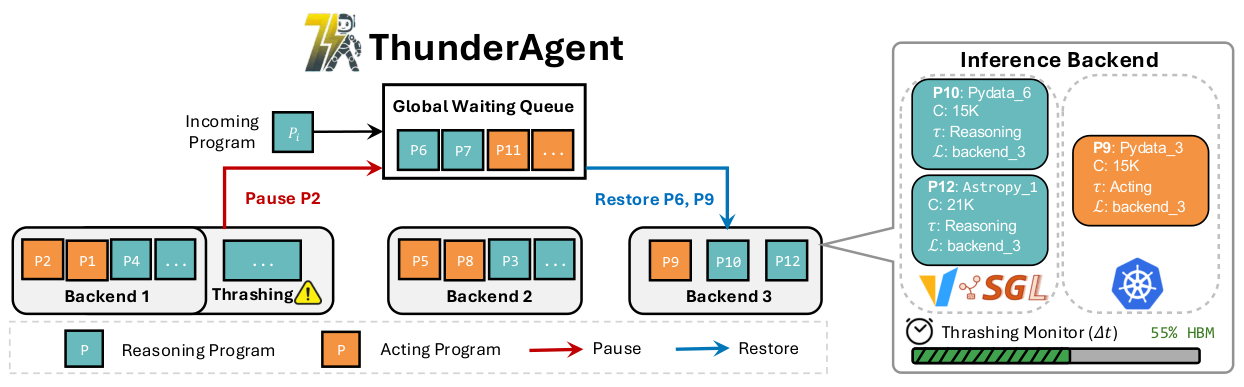
\includegraphics[width=\linewidth]{figures/papers/thunderagent-overview.png}
\caption{ThunderAgent's original system overview, showing program-aware
coordination of inference and tool execution. Reproduced from Kang et
al.~\cite{thunder}, Figure 3, arXiv:2602.13692v3, CC BY 4.0; scaled only.}
\label{fig:thunder-original}
\end{figure}

These systems also bound the research claim. If a simple robust TTL, native
retention priority, or working-set policy captures most of the benefit, a more
complex predictor may not be worth its cost. The right experiment asks what
extra information changes a decision, not whether the system beats an
intentionally oblivious baseline.

\section{Where ATFM fits, and what would make it useful}
\label{sec:atfm}
\subsection{The specific information advantage being proposed}
ATFM observes session/tool events, maintains a live forecast board, and turns
forecasts into admission or placement-related directives. Its potential
advantage is \emph{lead time}: a tool-progress update may reveal a return before
a gateway sees the next LLM request. A router choosing among destinations for
an already-arrived prompt solves a different timing problem, although modern
routing and scaling systems already use predictive models.

\fig{atfm}{0.97}{ATFM's conceptual feedback loop. Forecasts become bounded
control decisions; observed outcomes must validate that decisions were delivered
and useful. Cache actuation is backend-dependent and is not depicted as a
universal direct GPU pin.}{atfm}

The candidate contribution has three parts: conditional forecasts from
session-specific observations; aggregate resource uncertainty rather than only
mean request rate; and decisions made early enough to affect future contention.
Each must earn its complexity. A high-quality forecast delivered after the
request arrives has no prefetch lead-time advantage. A prediction that changes
no action has no decision value. An action that increases another tenant's
latency more than it saves may be undesirable even when the forecast is correct.

The architecture suggests a useful separation. Keep the request path bounded
and capable of falling back. Run heavier forecasting on snapshots or an
independently budgeted path. Deliver versioned, expiring decisions to actuators
that own the affected resource. This is a design direction; it must not be
mistaken for a claim that every isolation and acknowledgement mechanism is
already implemented.

\subsection{Admission constraints: population risk and sample risk}
For resource $r$ in slot $s$, let $Y_{rs}$ be uncertain protected demand,
$a_{is}$ a binary assignment of background job $i$, and $d_{ir}$ its estimated
demand. A conceptual marginal chance constraint is
\begin{equation}
 \Prb\!\left(Y_{rs}+\sum_i a_{is}d_{ir}\le C_{rs}\right)
 \ge1-\epsilon_{rs}.
 \label{eq:chance}
\end{equation}
Capacity $C_{rs}$ must use the same units and time interpretation as demand.
Existing resident KV and future arriving KV are not interchangeable. A system
that imposes separate resource constraints does not automatically have a joint
$1-\epsilon$ guarantee across resources and slots. A conservative union bound
allocates risks so $\sum_{r,s}\epsilon_{rs}\le\epsilon_{\mathrm{joint}}$;
a joint-scenario method is another option.

With $K$ forecast samples, a planner can evaluate
\begin{equation}
 \frac1K\sum_{k=1}^K\ind\left\{Y_{rs}^{(k)}+\sum_i a_{is}d_{ir}\le C_{rs}\right\}
 \ge1-\epsilon_{rs}.
\end{equation}
This is an empirical constraint under the forecast sample distribution. It is
not automatically a frequentist guarantee for true future traffic. Finite
sample uncertainty, model error, drift, and correlated residuals all matter.
As a simple illustration, even for independent correctly generated draws, a
Bernoulli event with probability 0.1 has estimated-probability standard error
$\sqrt{0.1\cdot0.9/256}\approx0.0188$ at 256 samples. Increasing samples reduces
Monte Carlo noise but does not correct model bias.

ATFM's GDP planner assigns deferrable work in forecast order using sampled
resource thresholds, bounded holds, and tenant-delay limits. Delay caps can
release work even when the capacity test has no feasible slot. Consequently
this implementation should be described as a bounded-delay heuristic with
empirical feasibility checks, not a proof of overload prevention. The code and
its scaling notes state the mechanics; a deployable capacity model remains an
experimental responsibility.

\subsection{A worked use case and its failure cases}
Imagine a worker pool near a latency limit. Several background agents are
running tests; an interactive user is generating a response. Some agents report
that their tests are nearly complete and will soon return with long contexts.
If this information is reliable and arrives early, a controller could defer
new deferrable tool launches, preserve selected cache state, or prepare capacity.
The objective is to reduce the coming peak, not to speed up the tests or invent
more GPU capacity.

Now change the assumptions. If the tests emit misleading progress, the
controller can hold unrelated work unnecessarily. If the contexts are small,
prefetch/control overhead can exceed the saved prefill. If the engine has ample
headroom, delaying anything may only increase completion time. If link bandwidth
is saturated, prefetching the predicted burst can congest it earlier. If an
existing TTL policy already retains the right prefixes, the extra forecast may
be redundant. If tool time dominates each job, a per-call latency improvement
may have negligible job-level impact.

A useful deployment region therefore requires all of the following to some
degree: repeated state, scarce resources, exploitable advance information,
a supported actuator, and a benefit greater than control/interference costs.
The size of that region is an empirical question. It cannot be established by
showing that one regression predicts durations accurately.

\subsection{Comparison by responsibility, not headline speedup}
\begin{longtable}{@{}p{0.18\linewidth}p{0.35\linewidth}p{0.40\linewidth}@{}}
\caption{Relevant systems and the comparison ATFM needs. Descriptions refer to
cited mechanisms, not a claim that other systems cannot be extended.}\label{tab:landscape}\\
\toprule System & Established focus & What an ATFM comparison must isolate\\\midrule
\endfirsthead
\toprule System & Established focus & What an ATFM comparison must isolate\\\midrule
\endhead
vLLM & Engine scheduling, paged state, prefix reuse & Incremental benefit on a tuned engine with native reuse enabled\\
SGLang / HiCache & Program execution, radix reuse, cache tiers & Extra value over existing match/prefetch/eviction policies\\
TensorRT-LLM & Optimized execution, reuse and retention controls & Prediction benefit beyond available native priorities\\
LMCache & State retention, movement, cross-engine reuse & Which supported operation a forecast improves, including its cost\\
Sarathi-Serve & Chunked prefill and phase interference & Admission benefit after reasonable intra-engine scheduling\\
DistServe & Separate prefill/decode resource allocation & Whether forecast value survives transfer and pool queueing\\
Mooncake & KV-centric distributed serving and overload control & Extra session information versus existing cluster policy\\
Preble & Distributed prefix reuse and load balancing & Anticipatory timing versus locality/load decisions at arrival\\
Dynamo & Routing, transfer coordination, scaling & Session-conditional signals beyond aggregate predictors\\
llm-d & Kubernetes inference routing and deployment composition & Integration ownership and comparison with enabled policies\\
Continuum & Bounded retention and program scheduling & Conditional forecasts versus robust TTL decisions\\
ThunderAgent & Program-aware inference and tool resources & Additional forecast value at equal workflow visibility\\
Tutti / AsymCache & IO- or kernel-aware cache optimization & Complementarity with a more efficient cache data path\\
ATFM prototype & Tool signals, sampled forecasts, bounded directives & End-to-end benefit remains to be established on real workers\\\bottomrule
\end{longtable}

\subsection{What the repository currently demonstrates}
This assessment is anchored to the repository at \texttt{900d63b}, not an
assumption that documentation implies hardware validation. Local source paths
are listed in Appendix~\ref{sec:code-map}.

\begin{itemize}
\item Offline trace adapters, session forecasting, Monte Carlo aggregation,
calibration, and evaluation are implemented. Recorded H1/H1b findings depend
on corpus, split, horizon, and signal quality.
\item The simulator contains queues, modeled workers, cache eviction, admission,
and placement-related comparisons. It permits controlled counterfactuals but
is not a real inference engine.
\item The board, proxy, event ingestion, and directive paths have local HTTP and
mock-worker integration evidence. A recorded Mocker setup lacked required KV
capacity metrics and issued no holds or touches; that run verifies wiring,
not the efficacy of those controls.
\item The LMCache HTTP adapter is tested against controlled responses. Current
controller compatibility, completed transfers, and actual GPU cache effects
remain unverified on the target deployment.
\item Tier and replica-floor proposals can be logged; the default launcher is
not evidence of a fully connected production autoscaler.
\item The completed refactor passed 420 tests with five skips. Deterministic
policy and forecast fixtures retained output hashes. This supports code
maintenance, not a GPU goodput or model-quality claim.
\end{itemize}

The status document also states that a completed H100 performance study is not
part of the recorded local evidence. The strongest useful present claim is that
ATFM provides a testable forecasting/control prototype with measured CPU and
integration behavior. Production serving advantage is still a hypothesis.

\subsection{Known control costs and the Python/Rust decision}
The repository has already removed repeated full-history JSONL scans, batched
hold delivery, introduced persistent admission heaps, and reduced planner and
empirical-sampling overhead. These changes target work volume before changing
implementation language. The following bounds distinguish independent scale
variables; there is no single meaningful $N$ for the whole system.

\begin{table}[htbp]\centering\small
\caption{Selected ATFM costs after the documented control refactors. Bounds omit
model-specific setup and external IO unless named.}
\begin{tabularx}{\linewidth}{@{}lXX@{}}\toprule
Operation & Principal scaling & Remaining qualification\\\midrule
Incremental log drain & $O(\Delta E)$ newly read bytes/records & First read and restart still replay retained history\\
Heap admission updates & Amortized $O(\log Q)$ per heap operation & Due timers and compaction can cause bursts\\
Peer rank hints & $O(U)$ distinct-index scan & Expected $O(1)$ count updates; $U \leq Q$\\
Batched hold transport & $\lceil D/B\rceil$ RPCs, $O(D)$ payload & No whole-plan distributed transaction\\
Monte Carlo aggregation & Depends on $N,K,H$; typically at least $O(NK)$ sample work & Vectorization does not eliminate samples or output arrays\\
GDP slot search & Range pruning; worst-case linear in eligible slots per job & Resource minima can occur in different slots\\\bottomrule
\end{tabularx}\end{table}

Here $\Delta E$ is newly appended event data, $Q$ queued requests, $D$ directives,
$B$ directives per transport batch, $N$ sessions, $K$ samples, and $H$ horizons.
Worst-case GDP work can be $O(NF)$ for $F$ eligible slots; if both grow together,
this is quadratic. Additional sample and resource dimensions belong explicitly
in threshold construction. An index does not guarantee a logarithmic search
when its pruning condition is only necessary. By contrast, returning a full
$Q$-element diagnostic snapshot necessarily costs $\Omega(Q)$.

Recent local proxy profiling found repeated runtime-detection import work and
removed it by supplying a missing serving dependency. Its paired fake-worker
trials improved latency/CPU in that configuration, but prediction timeout rates
increased. That result is recorded in the proxy-profiling report. It demonstrates
why a lower CPU total is not sufficient evidence of a healthier control loop.
The September 28 implementation bounds unfinished proxy prediction jobs (four
by default), falls back immediately at capacity, and keeps abandoned running
jobs counted until completion. A monotonic deadline spans dispatch and execution;
board HTTP phases use its remaining budget instead of a 500\,ms minimum.
Caller outcomes and actual unfinished work are counted separately. This bounds
local work, not remote computation or hard real-time response. It can exchange
timeouts for immediate rejection, so timely prediction use must be measured
alongside request latency. At that revision, synchronous board computation and remaining linear
rank work remained investigation targets.


The subsequent board-isolation implementation moves ingestion, forecasting and
planning to one bounded worker and publishes complete scalar prediction views.
Built-in HTTP predictions use expected $O(1)$ lookup; a per-tick projection costs
$O(S+D)$ for $S$ sessions and $D$ duration observations visited across distinct
means. A monotonic age limit includes computation time and triggers fallback
when the last completed view is too old. Quantiles and directive JSON are
prepared on the worker; numerical algorithms and seeded draw order are unchanged.
Threads still share the GIL. In three fresh paired 1,024-session trials, timely
prediction use rises from 24.59\% to 31.61\% and board heartbeat p95 delay falls
from roughly 90\,ms to 1--2\,ms. However, client p95 increases in every pair,
including three further pairs with zero hold delay. This is evidence for board
responsiveness and availability, not a serving-latency improvement. The dated
board-isolation report preserves the regression, raw evidence and host limits.

Python is currently appropriate for orchestration and numerical experimentation,
with bulk numerical work handled by compiled libraries. Rust becomes attractive
for a \emph{measured} high-frequency CPU component when algorithmic fixes,
batching, and boundary costs have already been addressed. A native module should
have a narrow contract and differential tests; moving the whole system would
add maintenance cost and could leave the real bottleneck unchanged. Transferring
large KV tensors and scheduling small metadata are separate costs, so neither
``Python is always negligible'' nor ``Rust will fix saturation'' is justified.

\subsection{An evaluation that could validate or reject the project}
\paragraph{Stage 1: establish executable contracts.}
Pin model, tokenizer/template, engine, cache connector, transport, and GPU
configuration. Verify the cache identity, supported retention/movement
operation, completion acknowledgement, expiration behavior, and observed
residency. Record whether the action protects GPU, CPU, disk, or a remote copy.
A mock endpoint returning 200 is insufficient. Test disconnects, stale events,
partial failures, and fallback; measure whether a retry changes the same object
or accidentally creates duplicate work.

\paragraph{Stage 2: evaluate forecasts without leakage.}
Split by complete session or workflow family and time, not arbitrary events
from the same run. Report residual-time calibration and quantile loss at
operational horizons. Compare aggregate last-value/rate predictors, age-only
survival, tool-type models, and progress-conditioned models. Include missing
progress, censored calls, unseen tools, and correlated backend slowdowns.
A forecaster may be well calibrated overall and systematically wrong for the
largest, most expensive contexts; stratify accordingly.

For quantile $q_\alpha$ and outcome $y$, pinball loss is
\begin{equation}
 L_\alpha(y,q_\alpha)=(\alpha-\ind\{y<q_\alpha\})(y-q_\alpha).
\end{equation}
Report empirical interval coverage as well as width. Narrow incorrect intervals
are not better forecasts. Evaluate service demand jointly with timing when they
are dependent, and retain deterministic seeds for parity tests without treating
seeds as independent production workloads.

\paragraph{Stage 3: isolate decision value.}
Use the same tuned engine and cache configuration across arms: native policy;
robust TTL/working-set baseline; aggregate forecasting; session age-only
forecasting; progress-conditioned ATFM; and an oracle whose extra information is
explicit. Disable individual actuators to separate admission, retention,
prefetch, and scaling effects. A simulated ``ThunderAgent-style'' policy must
not be labelled a benchmark of the full ThunderAgent implementation. Likewise,
a clairvoyant cache schedule is an upper bound under its modeled constraints,
not a deployable competitor.

\paragraph{Stage 4: run closed-loop agent workloads on real workers.}
Vary sessions, prompt/output lengths, tool gaps, shared-prefix fraction, cache
capacity, transfer bandwidth, burst correlation, tenant mix, and forecast error.
Include low load where control can only add overhead, near-saturation load where
it may help, and sustained overload where admission must make tradeoffs. Use
both reproducible synthetic programs and real tool traces. Preserve causal
turn dependencies so latency changes alter future arrival times correctly.

\paragraph{Stage 5: account for the entire outcome.}
Measure offered/completed/rejected work, joint-SLO goodput, TTFT, ITL tails,
whole-job completion, fairness, cache bytes by tier, useful/wasted transfers,
recomputed tokens, GPU idle time, controller CPU, queueing, and prediction
deadline misses. Include warmup, shutdown/drain rules, retries, errors, and
load-generator lateness. Run paired workloads with alternating order and
confidence intervals at the independent workload/run level. Correlated tokens
from one request are not independent experimental replicates.

\paragraph{Success and falsification criteria.}
A positive result should show an improved user-relevant objective at equal
resource budget, no unreported quality loss, and acceptable fairness/overhead.
A negative result is informative if simple TTL or native policies match the
benefit, useful lead time is scarce, prediction deadlines are missed, or cache
movement dominates savings. The project remains useful only if the value of
extra information survives the full path from observation to completed action.


\paragraph{Measured proxy follow-up.}
The next implementation study separates prediction, admission and dispatch
waiting and replaces per-release peer-list construction with exact per-tier
index counts. A rank query scans $U_t$ distinct queued indices; updates are
expected $O(1)$ and storage is $O(U)$ across tiers. The worst case still has
$U_t=Q$, so this does not eliminate quadratic total rank work across a unique
backlog. Strict ties and the admission policy are preserved.
Six paired local trials reduced proxy CPU in every pair, while client p95
improved in four and regressed in two. At 1,024 sessions, the per-run p95 ranges
were 2.564--4.067\,s before and 1.823--2.630\,s after; variability precludes a
single reliable speedup claim. A separate larger-connection-pool experiment
regressed large-case latency and was reverted, despite opening fewer TCP
connections. All 46,080 unprofiled calls across the two studies succeeded;
one instrumented pool trial was incomplete and is identified separately.
The repository's dated proxy-ranking report preserves source revisions and raw
evidence. These measurements concern CPU and HTTP overhead with a fake worker,
not inference throughput, GPU memory movement, or production capacity.


\paragraph{Transport isolation and bounded pools.}
The subsequent local study isolates HTTP transport from the board and admission
queue, then balances unfinished response lifetimes across 16 smaller pools with
a combined 100-connection cap. Selection costs $O(P)$ for $P$ pools; internal
HTTP scans remain, and requests are not migrated between shards. The aggregate
idle cap rises from 20 to 100 with unchanged expiry. One shared verifying TLS
context and stock fallback for HTTP proxy discovery preserve operational choices.
The small-load fixture regressed latency, so automatic selection retains stock
HTTPX for initial admission windows of 20 or fewer; larger windows select shards.

All six full-proxy pairs improved client p95 and proxy CPU. At 1,024 sessions,
p95 ranges changed from 2.462--2.654\,s to 1.422--1.465\,s. Timely prediction use
fell from 35.50\% to 31.93\%, with substantially more caller timeouts, so improved
transport latency is not evidence of improved forecasting or control quality.
All 23,040 full-proxy and 82,944 formal component requests succeeded. These short
localhost nonstreaming trials exclude real inference and network/TLS costs;
real-socket lifecycle tests do not establish streaming performance. The dated
sharded-transport study retains measured revisions, unfavorable small-case
results, the final automatic-selection distinction and raw evidence.

\clearpage

\appendix
\section{Notation and units}
\begin{longtable}{@{}p{0.19\linewidth}p{0.73\linewidth}@{}}
\toprule Symbol & Meaning\\\midrule\endfirsthead
\toprule Symbol & Meaning\\\midrule\endhead
$L,d,d_h$ & Layer count, hidden width, per-head dimension\\
$H_q,H_{kv}$ & Query heads and KV heads; they need not be equal\\
$T,U$ & Prompt/context length and number of generated output tokens\\
$b$ & Bytes per stored scalar; scales/metadata may be additional\\
$B$ & Active batch size in engine examples; directive batch size only in the explicitly defined ATFM table\\
$p$ & Tokens per physical cache block\\
$M_{\mathrm{KV}}$ & KV payload bytes, with sharding/replication specified separately\\
$P_{\mathrm{eff}}$ & Effective compute rate for the actual operations/shapes\\
$B_{\mathrm{effective}}$ & Effective bandwidth in bytes/s, not bits/s\\
$Q,N,K,H,F$ & Queued requests, sessions, Monte Carlo samples, forecast horizons, and candidate time slots\\
$R_i,D_{ir}$ & Session return time and its demand for resource $r$\\
$C_{rs}$ & Usable capacity for resource $r$ in slot $s$ under a stated model\\
$F(t),S(t),h(t)$ & CDF, survival function, and hazard of a duration/residual distribution\\
$\rho$ & Utilization under the simplified queue model\\
$\tau,\epsilon$ & A time/SLO bound and a probability-risk budget, respectively\\\bottomrule
\end{longtable}

A KiB is $2^{10}$ bytes and a GiB is $2^{30}$ bytes; a GB is $10^9$ bytes.
A 100 Gb/s link has a raw decimal byte rate of 12.5 GB/s before protocol and
implementation overhead, approximately 11.64 GiB/s. Do not substitute 100 GB/s
into a transfer equation for such a link. In the illustrations, bandwidth is
explicitly in GiB/s to match payload units. A model's advertised maximum context
length is a supported per-sequence limit, not a promise that many maximum-length
sequences fit or meet an SLO simultaneously.

\section{Terminology that is easy to conflate}
\begin{description}[style=nextline,leftmargin=0pt]
\item[KV cache versus response cache]
KV caches intermediate attention state. Response caching returns a previously
produced answer and requires its own semantic/freshness contract. Reusing KV can
still produce a different output sample.
\item[Prefix reuse versus session identity]
A session label is application metadata. Exact reuse depends on compatible
model state and prefix tokens. Two different sessions may share a prefix; two
requests in one session may lose reuse after editing earlier context.
\item[Cache hit versus ready state]
A metadata hit says an object is known at a location. Execution also requires
valid ownership, complete transfer, compatible layout, and synchronization.
\item[Eviction versus offload versus deletion]
Eviction removes an object from a tier's available resident set. Offload preserves
a representation elsewhere. Deletion removes the retained representation from
the relevant store. Exact meanings are API-specific.
\item[Pin versus priority versus touch]
A pin normally constrains eviction in a defined location. Priority changes
relative preference. A touch causes an access that may affect recency. They are
not interchangeable guarantees, and an external-store pin need not pin engine HBM.
\item[Continuous batching versus request concurrency]
Concurrency counts outstanding requests. Continuous batching chooses token work
between iterations. Large concurrency can increase queueing without increasing
useful device work.
\item[Prefill/decode disaggregation versus model parallelism]
Disaggregation separates request phases. Model parallelism splits one phase's
model execution across devices. They can be combined.
\item[Goodput versus throughput]
Throughput counts completed work under a chosen unit. Goodput counts work meeting
an explicit quality or latency condition. Both need the offered workload and
resource budget for interpretation.
\item[Prediction interval versus capacity guarantee]
A calibrated interval describes outcome frequency under an evaluated distribution.
It is not proof that a controller remains safe after arbitrary distribution
shift or that joint resource risks have been bounded.
\end{description}

\section{A complete example: one agent returning to a changed fleet}
This example is constructed for explanation. It is not a simulator result or a
measurement. Use the 128 KiB/token cache geometry from
Equation~\ref{eq:kvbytes}. An agent has an 8192-token prefix (1 GiB), finishes a
turn, and launches a tool. Another workload needs memory while it waits.

\begin{enumerate}
\item \textbf{At departure}, the engine releases active references according to
its policy. Retained blocks may remain reusable but evictable. An external cache
may also have a copy; do not assume one was written merely because offload is
configured.
\item \textbf{During the gap}, a progress update changes the predicted remaining
time to approximately two seconds with uncertainty. If a CPU copy exists, a
forecasting policy might arrange a restore shortly before the expected return.
It must include current transfer queueing and destination capacity.
\item \textbf{At arrival}, the tool result adds 512 tokens. A perfect old-prefix
hit still requires processing that suffix and its attention to prior context.
The full new payload at 8704 tokens is 1.0625 GiB, before output growth.
\item \textbf{At routing}, worker A has the old prefix but 200 ms of estimated
queueing. Worker B is idle but would pay an assumed 150 ms recomputation penalty.
Ignoring all other differences, B can win. If A's queue is only 20 ms, A can win.
Locality must be valued in time, not treated as an absolute preference.
\item \textbf{After a restore}, an operation acknowledgement must establish which
bytes became usable and where. If it only confirms admission to an asynchronous
transfer queue, the engine may still be unable to start.
\item \textbf{At evaluation}, compare job completion and other tenants' latency.
Saving this agent 150 ms while delaying ten others by 30 ms each may worsen a
sum-of-latencies objective. A class-weighted objective could prefer a different
choice; state those weights explicitly.
\end{enumerate}

A shared prefix further changes the accounting. If four sessions genuinely
share the same 1 GiB physical prefix, its retained payload is not 4 GiB. It can
also have higher reuse value than a private 1 GiB suffix. A session-level policy
that ignores block sharing can double-count memory and independently evict or
pin state whose ownership is shared. The actuator must reconcile these decisions
with the engine's object/block identities.

\section{A diagnosis guide for slow serving}
\begin{longtable}{@{}p{0.25\linewidth}p{0.31\linewidth}p{0.37\linewidth}@{}}
\toprule Symptom & Candidate explanation & Measurement that distinguishes it\\\midrule
\endfirsthead\toprule Symptom & Candidate explanation & Measurement that distinguishes it\\\midrule\endhead
High TTFT, low GPU busy time & Queueing outside engine, CPU dispatch, cache IO & Per-stage trace; frontend queue age; CPU/event-loop profile; transfer completion\\
High TTFT, heavy prefill work & Long prompts or poor prefix reuse & Uncached input tokens; cache identity/hit lengths; prefill kernel duration\\
Long ITL spikes & Prefill interference, collectives, pauses & Iteration composition; chunk size; device trace; per-token delivery timing\\
Frequent recompute/preemption & Active-state pressure or weak retention & Free/used blocks; eviction reason; prefix age; memory by owner\\
High hit rate but little benefit & Remote hits, short saved prefixes, hot worker & Saved compute time versus lookup/restore/queue time\\
Throughput plateaus with spare GPU & CPU/router/generator saturation & Per-process CPU, event-loop lag, offered versus delivered arrival rate\\
Good call latency, poor job latency & Tools, orchestration, serial dependencies & Whole-session critical-path trace and task-success metric\\
Prediction fallbacks rise at scale & Shared CPU or unbounded work backlog & Prediction deadline misses, queue age, cancellation effectiveness\\
Prefetch improves one class only & Transfer/memory interference or unfairness & Per-tenant latency and bandwidth; wasted prefetch and retention time\\\bottomrule
\end{longtable}

Use a profiler to locate time and an uninstrumented run to measure the effect
of a change. Instrumentation can distort short operations and asynchronous
scheduling. A fake worker is useful for isolating HTTP and controller overhead,
but cannot establish the balance of GPU kernels, HBM, collectives, and actual KV
transfers. Likewise, an offline maximum-throughput benchmark is not evidence
about an open arrival process under tail-latency constraints.

\section{Repository map and evidence trail}
\label{sec:code-map}
These paths are relative to the ATFM repository and identify the prototype's
implementation/evidence at the baseline revision. They are not upstream API
contracts. The repository is available at
\url{https://github.com/Alexander-Aghili/ATFM/tree/900d63b}.

{\small
\begin{longtable}{@{}p{0.43\linewidth}p{0.50\linewidth}@{}}
\toprule Path & Responsibility or evidence\\\midrule\endfirsthead
\toprule Path & Responsibility or evidence\\\midrule\endhead
\path{src/atfm/sidecar/} & Tool execution, progress extraction, configuration, harness adapters\\
\path{src/atfm/board/} & Session state, forecasts, predictors, aggregation, live HTTP board\\
\path{src/atfm/proxy/queue.py} & Persistent admission indexes and timed release\\
\path{src/atfm/control/gdp.py} & Bounded-delay slot assignment and empirical resource tests\\
\path{src/atfm/control/touch.py} & Budgeted touches and tier recommendations\\
\path{src/atfm/control/lmcache.py} & Configurable HTTP actuator; current upstream compatibility remains open\\
\path{src/atfm/sim/} & Modeled engine and policy comparisons\\
\path{experiments/} & CPU, serving, forecasting, and profiling studies outside the core package\\
\path{docs/status.md} & Implemented versus validated capabilities\\
\path{docs/development/control-scaling.md} & Algorithms, exact contracts, complexity, retained benchmarks\\
\path{docs/research/2026-09-27-proxy-profiling.md} & Proxy profiles, dependency correction, latency and timeout tradeoffs\\
\path{docs/research/2026-09-28-core-refactor.md} & Refactor decisions, parity hashes, timing limits, final tests\\
\path{docs/paper/control-implementation.tex} & Main research paper's control implementation/evidence section\\
\path{docs/research/2026-09-29-public-gpu-workloads.md} & First H100 NVL public-trace replays and BFCL checks (later revision)\\
\path{docs/research/2026-09-29-gpu-round2.md} & Complete 119-request root, 24/48\,GiB CPU tier, A100 repeats (later revision)\\
\path{docs/research/2026-09-30-gpu-round3.md} & Randomized capacity and chunk repeats, Blackwell (later revision)\\
\path{docs/research/2026-09-30-retrieval-paths.md} & Stage C cold, L2 and warmed-L1 retrieval paths (later revision)\\\bottomrule
\end{longtable}
}

The background paper intentionally has its own source, figures, and bibliography.
It can be rebuilt without rewriting the main research manuscript or its frozen
results. Original architecture diagrams are editable reladraw files. Mathematical
plots are generated by \path{plots.py}; \path{illustration-inputs.json} records
assumptions. No illustration should be relabelled as experimental evidence.
The one measured figure (Figure~\ref{fig:retrieval}) is generated separately by
\path{evidence_plots.py} from \path{measured-evidence.json}, which transcribes
the stage C report's medians and names its source.

\section{Reading sequence and open questions}
A productive sequence is: attention and GQA for the representation; Orca and
PagedAttention for scheduling and allocation; Sarathi-Serve and DistServe for
phase interference; SGLang/HiCache, LMCache, and Mooncake for reuse and movement;
Preble, Dynamo, and llm-d for fleet composition; then Continuum and ThunderAgent
for the direct agent-scheduling comparison. Read the relevant current project
documentation before implementing an integration: a paper explains a design,
but does not pin today's connector or controller API.

Three questions now connect this background to a falsifiable research plan:
does progress improve forecasts at actionable lead times; can a real actuator
convert those forecasts into ready-state advantages without displacing more
valuable work; and does that advantage improve goodput or job completion over
strong baselines after control costs and fairness are included?

\clearpage
\phantomsection\addcontentsline{toc}{section}{References}
{\small\begin{thebibliography}{99}

\bibitem{transformer} Vaswani et al.. \emph{Attention Is All You Need}. 2017. \url{https://arxiv.org/abs/1706.03762}. Accessed 28 September 2026.

\bibitem{mqa} Shazeer. \emph{Fast Transformer Decoding: One Write-Head is All You Need}. 2019. \url{https://arxiv.org/abs/1911.02150}. Accessed 28 September 2026.

\bibitem{gqa} Ainslie et al.. \emph{GQA: Training Generalized Multi-Query Transformer Models from Multi-Head Checkpoints}. 2023. \url{https://arxiv.org/abs/2305.13245}. Accessed 28 September 2026.

\bibitem{flash} Dao et al.. \emph{FlashAttention: Fast and Memory-Efficient Exact Attention with IO-Awareness}. 2022. \url{https://arxiv.org/abs/2205.14135}. Accessed 28 September 2026.

\bibitem{flash3} Shah et al.. \emph{FlashAttention-3: Fast and Accurate Attention with Asynchrony and Low-precision}. 2024. \url{https://arxiv.org/abs/2407.08608}. Accessed 28 September 2026.

\bibitem{flashinfer} Ye et al.. \emph{FlashInfer: Efficient and Customizable Attention Engine for LLM Inference Serving}. 2025. \url{https://arxiv.org/abs/2501.01005}. Accessed 28 September 2026.

\bibitem{orca} Yu et al.. \emph{Orca: A Distributed Serving System for Transformer-Based Generative Models}. 2022. \url{https://www.usenix.org/conference/osdi22/presentation/yu}. Accessed 28 September 2026.

\bibitem{paged} Kwon et al.. \emph{Efficient Memory Management for Large Language Model Serving with PagedAttention}. 2023. \url{https://arxiv.org/abs/2309.06180}. Accessed 28 September 2026.

\bibitem{v1} vLLM contributors. \emph{vLLM V1 guide}. living documentation. \url{https://github.com/vllm-project/vllm/blob/main/docs/usage/v1_guide.md}. Accessed 28 September 2026.

\bibitem{prefix} vLLM contributors. \emph{Automatic Prefix Caching}. v0.15.0 documentation. \url{https://docs.vllm.ai/en/v0.15.0/design/prefix_caching/}. Accessed 28 September 2026.

\bibitem{hybrid} vLLM contributors. \emph{Hybrid KV Cache Manager}. living documentation. \url{https://docs.vllm.ai/en/latest/design/hybrid_kv_cache_manager/}. Accessed 28 September 2026.

\bibitem{vdisagg} vLLM contributors. \emph{Disaggregated Prefilling (experimental)}. v0.20.0 documentation. \url{https://docs.vllm.ai/en/v0.20.0/features/disagg_prefill/}. Accessed 28 September 2026.

\bibitem{sglang} Zheng et al.. \emph{SGLang: Efficient Execution of Structured Language Model Programs}. 2023. \url{https://arxiv.org/abs/2312.07104}. Accessed 28 September 2026.

\bibitem{hicache} SGLang contributors. \emph{HiCache System Design and Optimization}. living documentation. \url{https://docs.sglang.io/docs/advanced_features/hicache_design}. Accessed 28 September 2026.

\bibitem{trt} NVIDIA. \emph{TensorRT-LLM KV Cache System}. living documentation. \url{https://nvidia.github.io/TensorRT-LLM/latest/features/kvcache.html}. Accessed 28 September 2026.

\bibitem{vattention} Prabhu et al.. \emph{vAttention: Dynamic Memory Management for Serving LLMs without PagedAttention}. 2024. \url{https://arxiv.org/abs/2405.04437}. Accessed 28 September 2026.

\bibitem{sarathi} Agrawal et al.. \emph{Taming Throughput-Latency Tradeoff in LLM Inference with Sarathi-Serve}. 2024. \url{https://arxiv.org/abs/2403.02310}. Accessed 28 September 2026.

\bibitem{distserve} Zhong et al.. \emph{DistServe: Disaggregating Prefill and Decoding for Goodput-optimized Large Language Model Serving}. 2024. \url{https://arxiv.org/abs/2401.09670}. Accessed 28 September 2026.

\bibitem{mooncake} Qin et al.. \emph{Mooncake: A KVCache-centric Disaggregated Architecture for LLM Serving}. 2025 revision. \url{https://arxiv.org/abs/2407.00079v4}. Accessed 28 September 2026.

\bibitem{preble} Srivatsa et al.. \emph{Preble: Efficient Distributed Prompt Scheduling for LLM Serving}. 2024. \url{https://arxiv.org/abs/2407.00023v2}. Accessed 28 September 2026.

\bibitem{lmcache} Cheng et al.. \emph{LMCache: An Efficient KV Cache Layer for Enterprise-Scale LLM Inference}. 2025. \url{https://arxiv.org/abs/2510.09665}. Accessed 28 September 2026.

\bibitem{lmp} LMCache contributors. \emph{Architecture and Developer Guide: multiprocess mode}. living documentation. \url{https://docs.lmcache.ai/mp/architecture.html}. Accessed 28 September 2026.

\bibitem{llegacy} LMCache contributors. \emph{LMCache Controller}. legacy documentation. \url{https://docs.lmcache.ai/kv_cache_management/index.html}. Accessed 28 September 2026.

\bibitem{lpin} LMCache contributors. \emph{Pin the KV cache}. legacy documentation. \url{https://docs.lmcache.ai/kv_cache_management/pin.html}. Accessed 28 September 2026.

\bibitem{cachegen} Liu et al.. \emph{CacheGen: KV Cache Compression and Streaming for Fast Large Language Model Serving}. 2023. \url{https://arxiv.org/abs/2310.07240}. Accessed 28 September 2026.

\bibitem{cacheblend} Yao et al.. \emph{CacheBlend: Fast Large Language Model Serving for RAG with Cached Knowledge Fusion}. 2025 revision. \url{https://arxiv.org/abs/2405.16444v3}. Accessed 28 September 2026.

\bibitem{kivi} Liu et al.. \emph{KIVI: A Tuning-Free Asymmetric 2bit Quantization for KV Cache}. 2024. \url{https://arxiv.org/abs/2402.02750}. Accessed 28 September 2026.

\bibitem{mla} DeepSeek-AI. \emph{DeepSeek-V2: A Strong, Economical, and Efficient Mixture-of-Experts Language Model}. 2024. \url{https://arxiv.org/abs/2405.04434}. Accessed 28 September 2026.

\bibitem{spec} Leviathan et al.. \emph{Fast Inference from Transformers via Speculative Decoding}. 2022. \url{https://arxiv.org/abs/2211.17192}. Accessed 28 September 2026.

\bibitem{dynamo} NVIDIA. \emph{Dynamo Architecture}. living documentation. \url{https://docs.nvidia.com/dynamo/dev/knowledge-base/concepts/architecture}. Accessed 28 September 2026.

\bibitem{drouter} NVIDIA. \emph{Dynamo KV-Aware Routing}. living documentation. \url{https://docs.nvidia.com/dynamo/dev/knowledge-base/concepts/system-architecture/kv-aware-routing}. Accessed 28 September 2026.

\bibitem{dplanner} NVIDIA. \emph{Dynamo Planner}. living documentation. \url{https://docs.nvidia.com/dynamo/dev/knowledge-base/modular-components/planner/overview}. Accessed 28 September 2026.

\bibitem{llmd} llm-d contributors. \emph{llm-d Architecture}. v0.9 documentation snapshot. \url{https://llm-d.ai/docs/architecture}. Accessed 28 September 2026.

\bibitem{continuum} Li et al.. \emph{Continuum: Efficient and Robust Multi-Turn LLM Agent Scheduling with KV Cache Time-to-Live}. 2026 revision. \url{https://arxiv.org/abs/2511.02230v7}. Accessed 28 September 2026.

\bibitem{thunder} Kang et al.. \emph{ThunderAgent: A Simple, Fast and Program-Aware Agentic Inference System}. 2026 revision. \url{https://arxiv.org/abs/2602.13692v3}. Accessed 28 September 2026.

\bibitem{tutti} Qiu et al.. \emph{Tutti: Making SSD-Backed KV Cache Practical for Long-Context LLM Serving}. 2026 preprint. \url{https://arxiv.org/abs/2605.03375}. Accessed 28 September 2026.

\bibitem{asym} Shi et al.. \emph{Multi-Segment Attention: Enabling Efficient KV-Cache Management for Faster Large Language Model Serving}. 2026 preprint. \url{https://arxiv.org/abs/2606.02964}. Accessed 28 September 2026.

\bibitem{agentbench} Chang et al.. \emph{From LLM Inference to Agentic Workloads: Characterization and Implications for Serving Systems}. 2026 preprint. \url{https://arxiv.org/abs/2608.15127}. Accessed 28 September 2026.

\bibitem{mlperf} MLCommons. \emph{Agentic Inference for MLPerf Inference}. 8 July 2026. \url{https://mlcommons.org/2026/07/agentic-inference-for-mlperf-inference/}. Accessed 28 September 2026.

\end{thebibliography}
}
\end{document}
